%Supplementary Information for the 2015 submission to Geophysical Research Letters with Jesse Day, Jake Edman, John Chiang, Inez Fung and Weihan Liu



%%%%%%%%%%%%%%%%%%%%%%%%%%%%%%%%%%%%%%%%%%%%%%%%%%%%%%%%%%%%%%%%%%%%%%%%%%%%
% AGUtmpl.tex: this template file is for s formatted with LaTeX2e,
% Modified November 2013
%
% This template includes commands and instructions
% given in the order necessary to produce a final output that will
% satisfy AGU requirements.
%
% PLEASE DO NOT USE YOUR OWN MACROS
% DO NOT USE \newcommand, \renewcommand, or \def.
%
% FOR FIGURES, DO NOT USE \psfrag
%
%%%%%%%%%%%%%%%%%%%%%%%%%%%%%%%%%%%%%%%%%%%%%%%%%%%%%%%%%%%%%%%%%%%%%%%%%%%%
%
% All questions should be e-mailed to latex@agu.org.
%
%%%%%%%%%%%%%%%%%%%%%%%%%%%%%%%%%%%%%%%%%%%%%%%%%%%%%%%%%%%%%%%%%%%%%%%%%%%%
%
% Step 1: Set the \documentclass
%
% There are two options for article format: two column (default)
% and draft.
%
% PLEASE USE THE DRAFT OPTION TO SUBMIT YOUR PAPERS.
% The draft option produces double spaced output.
%
% Choose the journal abbreviation for the journal you are
% submitting to:

% jgrga JOURNAL OF GEOPHYSICAL RESEARCH
% gbc   GLOBAL BIOCHEMICAL CYCLES
% grl   GEOPHYSICAL RESEARCH LETTERS
% pal   PALEOCEANOGRAPHY
% ras   RADIO SCIENCE
% rog   REVIEWS OF GEOPHYSICS
% tec   TECTONICS
% wrr   WATER RESOURCES RESEARCH
% gc    GEOCHEMISTRY, GEOPHYSICS, GEOSYSTEMS
% sw    SPACE WEATHER
% ms    JAMES
% ef    EARTH'S FUTURE
%
%
%
% (If you are submitting to a journal other than jgrga,
% substitute the initials of the journal for "jgrga" below.)

\documentclass[draft,grl]{agutexSI}

\usepackage{hyperref}
\usepackage{rotating}
\usepackage{amsmath}


%%%%%%%%%%%%%%%%%%%%%%%%%%%%%%%%%%%%%%%%%%%%%%%%%%%%%%%%%%%%%%%%%%%%%%%%%
%
%  SUPPORTING INFORMATION TEMPLATE
%
%% ------------------------------------------------------------------------ %%
%
%
%Please use this template when formatting and submitting your Supporting Information.

%This template serves as both a “table of contents” for the supporting information for your article and as a summary of files.
%
%
%OVERVIEW
%
%Please note that all supporting information will be peer reviewed with your manuscript.
%In general, the purpose of the supporting information is to enable authors to provide and archive auxiliary information such as data %tables, method information, figures, video, or computer software, in digital formats so that other scientists can use it.
%The key criteria are that the data:
% 1. supplement the main scientific conclusions of the paper but are not essential to the conclusions (with the exception of
%    including %data so the experiment can be reproducible);
% 2. are likely to be usable or used by other scientists working in the field;
% 3. are described with sufficient precision that other scientists can understand them, and
% 4. are not exe files.
%
%USING THIS TEMPLATE
%
%All Supporting text and figures should be included in this document. Insert supporting information content into each appropriate section of the template. %Figures and tables should appear above each caption.  To add additional captions, simply copy and paste each sample caption as needed.

%Tables may be included, but can also be uploaded separately, especially if they are larger than 1 page, or if necessary for retaining table formatting. Data sets, large tables, movie files, and audio files should be uploaded separately, following AGU naming conventions. Include their captions in this document and list the file name with the caption. You will be prompted to upload these files on the Upload Files tab during the submission process, using file type “Supporting Information (SI)”

%IMPORTANT NOTE ON FIGURES AND TABLES
% Placeholders for figures and tables appear after the \end{article} command, after references.
% DO NOT USE \psfrag or \subfigure commands.
%
%  Uncomment the following command to include .eps files
 % \usepackage[dvips]{graphicx}
%
%  Uncomment the following command to allow illustrations to print
%   when using Draft:
%  \setkeys{Gin}{draft=false}
%
% Substitute one of the following for [dvips] above
% if you are using a different driver program and want to
% proof your illustrations on your machine:
%
% [xdvi], [dvipdf], [dvipsone], [dviwindo], [emtex], [dviwin],
% [pctexps],  [pctexwin],  [pctexhp],  [pctex32], [truetex], [tcidvi],
% [oztex], [textures]
%
%
%% ------------------------------------------------------------------------ %%
%
%  ENTER PREAMBLE
%
%% ------------------------------------------------------------------------ %%

% Author names in capital letters:
%\authorrunninghead{BALES ET AL.}

% Shorter version of title entered in capital letters:
%\titlerunninghead{SHORT TITLE}

%Corresponding author mailing address and e-mail address:
%\authoraddr{Corresponding author: A. B. Smith,
%Department of Hydrology and Water Resources, University of
%Arizona, Harshbarger Building 11, Tucson, AZ 85721, USA.
%(a.b.smith@hwr.arizona.edu)}

\begin{document}

%% ------------------------------------------------------------------------ %%
%
%  TITLE
%
%% ------------------------------------------------------------------------ %%

%\includegraphics{agu_pubart-white_reduced.eps}


\title{Supporting Information for ``Signature of the `South Flood-North Drought' Pattern in Meiyu Front and Tropospheric Jet Changes''}
%
% e.g., \title{Supporting Information for "Terrestrial ring current:
% Origin, formation, and decay $\alpha\beta\Gamma\Delta$"}
%
%DOI: 10.1002/%insert paper number here%

%% ------------------------------------------------------------------------ %%
%
%  AUTHORS AND AFFILIATIONS
%
%% ------------------------------------------------------------------------ %%


%Use \author{\altaffilmark{}} and \altaffiltext{}

% \altaffilmark will produce footnote;
% matching \altaffiltext will appear at bottom of page.


\authors{Jesse A. Day\altaffilmark{1},
Jacob P. Edman\altaffilmark{1}, John C. H. Chiang\altaffilmark{2}, Inez Fung \altaffilmark{1}, and
Weihan Liu\altaffilmark{3}}

\altaffiltext{1}{Department of Earth and Planetary Science, University of California Berkeley, Berkeley, California, USA.}
\altaffiltext{2}{Department of Geography, University of California Berkeley, Berkeley, California, USA.}
\altaffiltext{3}{College of Letters and Science, University of California Berkeley, Berkeley, California, USA.}



%% ------------------------------------------------------------------------ %%
%
%  BEGIN ARTICLE
%
%% ------------------------------------------------------------------------ %%

% The body of the article must start with a \begin{article} command
%
% \end{article} must follow the references section, before the figures
%  and tables.

\begin{article}

%% ------------------------------------------------------------------------ %%
%
%  TEXT
%
%% ------------------------------------------------------------------------ %%


\noindent\textbf{Contents of this file}
%%%Remove or add items as needed%%%
\begin{enumerate}
\item Text S1 to S2
We include a more comprehensive description of several algorithms used in the text, including a description of bootstrapping methods used and of the kernel method used for plotting jet density in main text Figures 3 and 4.

\item Figures S1 to Sx
We include five figures. Figure S1 demonstrates the functionality of the Front Detection algorithm by showing different cases of its operation. Figure S2 plots a climatology of the average quality scores of accepted frontal events throughout the year. Figure S5 shows the autocorrelation of daily mean jet latitude in order to justify the use of the bootstrap Kolmogorov-Smirnov method with jet data drawn in blocks.

\item Tables S1 to S6
We include six tables. Tables S1-S3 detail various aspects of the functionality of the front detection algorithm. Table S4 shows the climatological properties of the Meiyu Front during different time periods. Table S5 shows the changes in these statistics in 1980-2007 versus 1951-1979, with statistically significant changes indicated. Table S6 shows the same properties as Table S2, but for 1994-2007 versus 1979-1993.
%if Tables are larger than 1 page, upload as separate excel file

\end{enumerate}
\noindent\textbf{Additional Supporting Information (Files uploaded separately)}
\begin{enumerate}
\item Captions for Datasets S1 to Sx
\end{enumerate}

%Type or paste your text here. The introduction gives a brief overview of the supporting information. You should include information %about as many of the following as possible (when appropriate):
% 1. a general overview of the kind of data files;
% 2. information about when and how the data were collected or created;
% 3. a general description of processing steps used;
% 4. any known imperfections or anomalies in the data.

\noindent\textbf{Introduction}
In this appendix, we provide more information about the workings of the novel recursive image processing algorithm used to compile statistics of frontal in China for 57 years based on the APHRODITE rain gauge data set \citep{Yatagai2012}. Furthermore, we include the results of the algorithm for different periods of interest, and relay the changes in frontal properties between the periods 1951-1979 and 1980-2007, which is the focus of the manuscript. We have also included a table of changes between the periods 1979-1993 and 1994-2007, which have been described in previous work and are different in nature from those described in Table S1. We also provide more information on the bootstrapping algorithms used to calculate statistical significance, as well as the kernel method used to estimate a density map of jet observations from discrete observations.

\clearpage

\noindent\textbf{Meiyu database}
We have made the full database of Meiyu statistics from January 1 1951 to December 31 2007 available at the author's personal website: \url{http://www.atmos.berkeley.edu/~jessed/mydata.html}

%Repeat for any additional Supporting data sets

\noindent\textbf{Jet database}
The kernel density contours shown in the main text (Figure 4) are derived from the jet counts of \citet{Schiemann2009} in the following way. First, we aggregate all the jet counts in the chosen time period (e.g. for 4b, we aggregate counts from days 121-160 for 1958-1979 and 1980-2001 separately). This results in a gridded histogram of the total number of jet counts, spanning 16.75-58.25 N and 42.5-130 E with 0.25x0.25 degree resolution. To estimate the kernel density, we use the function 'bke2d' from the R package `KernSmooth,' which produces a binned kernel density estimate using the standard bivariate normal distribution. This gives an estimate of the probability density function of jet location in a given time period. 

\clearpage

\noindent\textbf{Front Algorithm}
The following text contains a full description of the recursively convergent algorithm used to find fronts in daily rainfall over China. The overall strategy is to find a single line corresponding to the strongest rainband on a given day (a ``primary'' front), and then to search for a potential additional rainband (a ``secondary front'') by removing all rainfall associated with the primary feature. In addition, we provide figures showing different cases of algorithm functionality.

\noindent\textbf{Recursive Fit}

\begin{enumerate}
	\item For a given day of accumulated rainfall over the longitudes 105-123$^{\circ}$E and 20-40$^{\circ}$N at $.25^{\circ}$ by $.25^{\circ}$ resolution, the first criterion is to check for a band of coherent rainfall maxima. The maximum daily rainfall at each longitude is found. If there exists a $5^{\circ}$ continuous chain of maxima (20 points in a row) exceeding 10 mm day$^{-1}$, we proceed to step 2 and attempt a fit (Figure S1a). Otherwise, no fit is attempted for that day (Figure S1b).
	
	\item A weighted least-squares linear fit of the \textit{latitudes} of the maxima is attempted in MATLAB using the intensity of the maxima as weight, with the goal of finding a linear front. To encourage convergence, the weight of outlying points is set to zero, where an outlier is defined as any maximum that is over $5^{\circ}$ from the \textit{centroid} of the precipitation maxima, calculated by $\left<lat_{max}\right>=\frac{\sum_{long} lat_{max}*max}{\sum_{long} \max}$ (Figure 1c). 
	
	\item A recursive algorithm converges on a best estimate. In each iteration, we find a new set of maxima within \textit{k} degrees of the previous best fit line, and again perform a weighted linear fit of the maxima. $k$ is progressively decreased with each iteration from $5^{\circ}$ to $2^{\circ}$ by $.25^{\circ}$ increments, and then from $2^{\circ}$ to $.25^{\circ}$ by $.25^{\circ}$ increments but repeating each width $k$ twice in a row. The fit obtained in the final iteration is taken as our best estimate of front position.
	
	\item We define the ``quality score'' $Q$ as the fraction of total daily precipitation inside of 105-123$^{\circ}$E and 20-40$^{\circ}$N that falls within $2.5^{\circ}$ degrees of the best estimate line. We also define intensity as mean rainfall at all points along the front axis where daily rainfall exceeds 5 mm day$^{-1}$ (``front points''), length as the total number of front points, and width as the mean distance between half-maxima (in degrees of latitude) on either side of each front point.
	
	\item Given an estimate of primary front position, we check for a secondary front. We start by removing all precipitation associated with the primary frontal event from our daily rainfall map. To do this, all rainfall within 4$^{\circ}$ of our primary front is set to 0, as are all other adjacent points where rainfall exceeds 10 mm day$^{-1}$ (Figure S1?). We then reapply the continuous maximum criterion from step 1. If passed, steps 2-4 are repeated to find a best estimate for the position of the secondary front, and secondary front attributes are calculated.
	
	\item If a secondary front is found, two additional quality scores $Q_1$ and $Q_2$ are calculated. $Q_1$ is defined as the fraction of rainfall contained in the primary front \textit{after removing all rainfall associated with the secondary front}. Likewise $Q_2$ is the Q score of the second front \textit{after removing all rainfall from the primary front}.		
	
\end{enumerate} 

In rare cases with two fronts of roughly equal strength but distant in latitude, the removal of outliers in step 2 prevents a fit entirely. We test for such cases by ensuring that the total sum of weights ${\sum_{long} max}$ exceeds 200 mm day$^{-1}$ (equivalent to our condition in bullet point 1). When this condition is failed, we return to step 1, but find maxima only over the latitude range 20N-$\left<lat_{max}\right>$ or $\left<lat_{max}\right>$-40N, depending on which half of our domain has a longer chain of maxima exceeding 10 mm day$^{-1}$, and subsequently proceed as usual.

\noindent\textbf{Quality Control}

After running the algorithm for all 20,819 days from 1 January 1951 to 31 December 2007, we obtained 11,228 frontal fits and 1,116 days with two fronts. Subsequently, we apply a quality control algorithm to eliminate days with poor fits. We define the quality scores $Q$, $Q_1$ and $Q_2$, and the ``Taiwan fraction'' (TW), defined as the percentage of daily rainfall inside the window 105-$123^{\circ}$E and 20-$40^{\circ}$N that falls on the island of Taiwan. We use these metrics to define the following two criteria for inclusion:

\begin{enumerate}

	\item If $TW > 20\%$, the day is thrown out (238 cases total, 2.1\% of total fits). Such days are dominated by a local storm reaching Taiwan and rarely exhibit a strong front.  
	
	\item Subsequently, a day can be included if it meets either of the following criteria:
	
	\begin{enumerate} 
	
	\item if $Q>.6$, the day is included in our statistics (7,522 days, 67.0\% of total fits). If $Q_2$ also is greater than .6, the day will be classified as a double front day (Type I double front; 232 cases, or 3.1\% of days where $Q>.6$).
		
	\item If $Q<.6$, a day can only be included if both $Q_1 \mathrm{\textbf{ and }} Q_2 > .6$ (where again Q1 and Q2 are \textit{conditional} quality scores as defined above). In such cases, the presence of multiple fronts of similar intensity initially obscures the quality of the fit. Such days are also classified as double front days (Type II double front; 466 cases). These statistics are also collectively repeated in supplementary tables S1-S3.
	
	\end{enumerate}
	
\end{enumerate}	
	
	The use of condition 2b adds 466 double front days that would otherwise have been categorized as days with no front, constituting 6.2\% of total days included in our statistics. 33.2\% of double front days are Type I and 66.8\% Type II. Double rainbands occur on 9.3\% of all days (698 out of 7,522 days), but are more common during certain seasons such as the Post-Meiyu (see Figure 1c in main text).
	
\clearpage

%%% TABLE 1 - ALGORITHM FUNCTIONALITY - BIG PICTURE
\begin{table}
\settablenum{S1} %%Change number for each table

\caption{Statistics on the functionality of the Front Detection algorithm. Number in parentheses indicates the percentage of days that fall into that category out of all 20,819 days.}
\centering

\begin{tabular}{ l c c c}
	  & Total Fits & Passes Quality Control & Percent Passing QC\\
	 \hline
	 Single & 11,228 (53.9\% of total) & 7,988 (38.4\% of total) & 71.1\% \\
	 Double & 1,116 (5.4\% of total) & 698 (3.4\% of total) & 62.5\% \\
\end{tabular}
\end{table}

%%% TABLE 2 - ALGORITHM FUNCTIONALITY - DETAILS, PRIMARY FRONT
\begin{table}
\settablenum{S2} %%Change number for each table

\caption{Details on the application of quality control criteria to primary front events.}
\centering

\begin{tabular}{ l c}
	 Criterion & Number (\% of total) \\
	 \hline
	 Primary Front days before QC & 11,228 \\
	 Taiwan days (TW$>20\%$) & 238 (2.1\%) \\
	 $Q>.6$ (strong front) & 7,522 (67.0\%) \\
	 Double front ($Q1>.6$ and $Q2>.6$) & 466 (4.2\%) \\
	 Poor fit (Fails QC) & 3008 (26.8\%) \\
	 
\end{tabular}
\end{table}

%%% TABLE 3 - ALGORITHM FUNCTIONALITY - DETAILS, SECONDARY FRONT
\begin{table}
\settablenum{S3} %%Change number for each table

\caption{Details on the application of quality control criteria to secondary front events.}
\centering

\begin{tabular}{ l c}
	 Criterion & Number (\% of total) \\
	 \hline
	 Secondary Front Days before QC & 1,116 \\
	 Type I fit ($Q>.6$ and $Q2>.6$) & 232 (20.8\%) \\
	 Type II fit ($Q1>.6$ and $Q2>.6$) & 466 (41.8\%) \\
	 Poor fit (Fails QC) & 418 (37.5\%) \\
	 
\end{tabular}
\end{table}

\clearpage

%%%% TABLE 4 - MEIYU STATISTICS %%%%
\noindent\textbf{Tables of Front Properties and Front Changes}

\begin{table}
\settablenum{S4} %%Change number for each table

\caption{Total number of rainbands as well as frequency of primary and secondary fronts, and the latitude and intensity of frontal rainbands during the Spring Rains, Pre-Meiyu, Meiyu season, Post-Meiyu, Fall Rains and for the full year. Statistics are compiled using both primary and secondary fronts, and are very close to results using primary fronts alone, except during the Post-Meiyu period when secondary fronts are common. Standard deviations for latitude and intensity are obtained by permutation (bootstrapping without replacement).}
\centering

\begin{tabular}{ l c c c c c c c}
	 \multicolumn{8}{c}{\textbf{1951-2007 Means}} \\
	 \textbf{Time Period} & $\boldsymbol{n}$ & $\boldsymbol{n_1}$ & \textbf{1f.} (\%) & $\boldsymbol{n_2}$ & \textbf{2f.} (\%) & \textbf{Lat} & \textbf{Int} (mm day$^{-1}$) \\
	 \hline
	\textbf{Spring Rains} (Mar 1-Apr 30, 60-120) & 1661 & 1635 & $47.0 \pm 0.8$ & 26 & $0.7 \pm 0.1$ & $27.5 \pm .1$ & $20.1 \pm .4$ \\
	\textbf{Pre-Meiyu} (May 1-Jun 9, 121-160) & 1371 & 1279 & $56.1 \pm 1.0$ & 92 & $4.0 \pm 0.4$ & $27.4 \pm .2$ & $25.5 \pm .5$ \\
	\textbf{Meiyu} (Jun 10-Jul 19, 161-120) & 1688 & 1499 &$65.8 \pm 1.0$ & 189 & $8.3 \pm 0.6$ & $29.5 \pm .2$ & $28.3 \pm .5$ \\
	\textbf{Post-Meiyu} (Jul 20-Sep 30) & 2113 & 1757 & $42.2 \pm 0.8 $ & 356 & $8.6 \pm 0.4$ & $29.9 \pm .2$ & $25.6 \pm .5$ \\
	\textbf{Post-Meiyu}, north of 27$^\circ$N & 1368 & 1215 & $27.1 \pm 0.7 $ & 153 & $3.4 \pm 0.3$ & $33.3 \pm .2$ & $23.9 \pm .5$ \\
	\textbf{Post-Meiyu}, south of 27$^\circ$N & 745 & 556 & $15.2 \pm 0.6 $ & 189 & $5.1 \pm 0.3$ & $23.7 \pm .1$ & $28.8 \pm .9$ \\
	\textbf{Fall Rains} (Oct 1-Nov 16) & 744 & 714 & $26.6 \pm 0.9 $ & 30 & $1.1 \pm 0.2$ & $29.2 \pm .3$ & $20.5 \pm .7$ \\
	\textbf{Full Year} (1-365) & 8682 & 7984 & $38.4 \pm 0.3$ & 698 & $3.4 \pm 0.1$ & $28.6 \pm .1$ & $23.5 \pm .2$ \\
\end{tabular}
\end{table}


%% TABLE 5 - change in front frequency between 1951-1979 and 1980-2007
\begin{table}
\settablenum{S5} %%Change number for each table

\centering

\caption{Change in frequency of primary fronts and secondary fronts between 1951-1979 and 1980-2007, with standard deviation of mean and p-value of change calculated analytically. Statistically significant changes at the 95\%/99\% level are indicated by bold/asterisk and bold.}

\begin{tabular}{ l c c c c c c}
	& \multicolumn{3}{c}{Primary front \%} & \multicolumn{3}{c}{Secondary front \%} \\
	\textbf{Period} & '51-'79 & '80-'07 & $p$ & '51-'79 & '80-'07 & $p$ \\
	\hline	
	\textbf{Spring Rains} (60-120)		& $46.4 \pm 1.2$ & $47.7 \pm 1.2$ & $ .77 $ 	& $0.8 \pm .2$ & $0.7 \pm .2$ & $.38$ \\
	\textbf{Pre-Meiyu} (121-160) 		& $\boldsymbol{59.0 \pm 1.4^*}$ & $\boldsymbol{53.0 \pm 1.5^*}$ & $ \boldsymbol{.0019^*} $ & $4.2 \pm .6$ & $3.8 \pm .6}$ & $.32$ \\
	\textbf{Meiyu} (161-200)			& $66.8 \pm 1.4$ & $64.6 \pm 1.4$ & $ .14 $ 	& $7.4 \pm .8$ & $9.2 \pm .9$  & $.94$ \\
	\textbf{Post-Meiyu} (201-273)		& $42.5 \pm 1.1$ & $42.0 \pm 1.1$ & $ .37 $	& $9.2 \pm .6$ & $7.8 \pm .6$ & $.049$ \\
	\textbf{Post-Meiyu}, $>27^\circ$N 	& $27.8 \pm 1.0$ & $26.4 \pm 1.0$ & $ .16 $ 	& $3.8 \pm .4$ & $2.9 \pm .4$ & $.047$ \\
	\textbf{Post-Meiyu}, $<27^\circ$N 	& $14.7 \pm 0.8 $ & $15.6 \pm 0.8$ & $ .78 $ 	& $5.4 \pm .5$ & $4.9 \pm .5$ & $.24$  \\
	\textbf{Fall Rains} (274-320)			& $25.8 \pm 1.2 $ & $27.6 \pm 1.2$ & $ .86 $ 	& $1.0 \pm .3$ & $1.2 \pm .3$ & $.68$ \\
	\textbf{Full Year} (1-365)			& $38.6 \pm 0.5 $ & $38.1 \pm 0.5$ & $ .25 $ 	& $3.4 \pm .2$ & $3.3 \pm .2$ & $.35$ \\

\end{tabular}
\end{table}

%% TABLE 6 - change in rainband latitude and intensity between 1951-1979 and 1980-2007
\begin{table}
\settablenum{S6} %%Change number for each table

\centering

\caption{Change in latitude and intensity of rainbands between 1951-1979 and 1980-2007, with standard deviation of mean and p-value of change both calculated by a permutation test with 10,000 iterations. Statistically significant changes at the 95\%/99\% level are indicated by bold/asterisk and bold.}

\begin{tabular}{ l c c c c c c}
	& \multicolumn{3}{c}{Front latitude ($^\circ$)} & \multicolumn{3}{c}{Intensity (mm day$^{-1})$} \\
	\textbf{Period} & '51-'79 & '80-'07 & $p$ & '51-'79 & '80-'07 & $p$ \\
	\hline	
	\textbf{Spring Rains} (60-120)		& $\boldsymbol{27.6 \pm .2}$ & $\boldsymbol{27.3 \pm .2}$ & $ \boldsymbol{.020} $ 		& $\boldsymbol{19.7 \pm .5}$ 	& $\boldsymbol{20.5 \pm .5} $ & $\boldsymbol{.984}$ \\
	\textbf{Pre-Meiyu} (121-160) 		& $27.5 \pm .3$ & $27.4 \pm .3$ & $ .29 $ 		& $25.4 \pm .7$ 	& $25.6 \pm .8	$ & $.72$ \\
	\textbf{Meiyu} (161-200)			& $29.6 \pm .3$ & $29.4 \pm .3$ & $ .24 $ 		& $28.2 \pm .8$ 	& $28.4 \pm .8	$  & $.71$ \\
	\textbf{Post-Meiyu} (201-273)		& $\boldsymbol{30.2 \pm .3^*}$ & $\boldsymbol{29.6 \pm .3^*}$ & $\boldsymbol{.0048^*} $	& $25.5 \pm .7$ 	& $25.7 \pm .7	$ & $.71$ \\
	\textbf{Post-Meiyu}, $>27^\circ$N 	& $\boldsymbol{33.6 \pm .2^*}$ & $\boldsymbol{32.9 \pm .3^*}$ & $\boldsymbol{.0003^*} $ 	& $23.5 \pm .7$ 	& $24.2 \pm .7	$ & $.92$ \\
	\textbf{Post-Meiyu}, $<27^\circ$N 	& $23.7 \pm .1 $ & $23.8 \pm .2$ & $ .83 $ 	& $29.1 \pm 1.3$ 	& $28.3 \pm 1.4	$ & $.20$  \\
	\textbf{Fall Rains} (274-320)			& $29.1 \pm .4 $ & $29.3 \pm .4$ & $ .79 $ 	& $20.3 \pm 1.0$ 	& $20.8 \pm .9	$ & $.76$ \\
	\textbf{Full Year} (1-365)			& $\boldsymbol{28.7 \pm .1 $^*} & $\boldsymbol{28.5 \pm .1 ^*}$ & $ \boldsymbol{.0032^*} $ 	& $23.3 \pm .3$ 	& $23.6 \pm .3	$ & $.95$ \\

\end{tabular}
\end{table}

%% TABLE 7 - change in front frequency between 1979-1993 and 1994-2007
\begin{table}
\settablenum{S7} %%Change number for each table

\centering

\caption{Change in frequency of primary fronts and secondary fronts between 1979-1993 and 1994-2007, with standard deviation of mean and p-value of change calculated analytically. Statistically significant changes at the 95\%/99\% level are indicated by bold/asterisk and bold.}

\begin{tabular}{ l c c c c c c}
	& \multicolumn{3}{c}{Primary front \%} & \multicolumn{3}{c}{Secondary front \%} \\
	\textbf{Period} & '79-'93 & '94-'07 & $p$ & '79-'93 & '94-'07 & $p$ \\
	\hline	
	\textbf{Spring Rains} (60-120)		& $50.0 \pm 1.7$ & $45.4 \pm 1.7$ & $ .029 $ 	& $0.9 \pm .3$ 	& $0.5 \pm .2$ & $.15$ \\
	\textbf{Pre-Meiyu} (121-160) 		& $53.0 \pm 2.0$ & $53.2 \pm 2.1$ & $ .53$ 	& $3.5 \pm .8$ 	& $4.1 \pm .8}$ & $.71$ \\
	\textbf{Meiyu} (161-200)			& $63.7 \pm 2.0$ & $64.8 \pm 2.0$ & $ .66 $ 	& $8.7 \pm 1.1$ 	& $9.5 \pm 1.2$  & $.68$ \\
	\textbf{Post-Meiyu} (201-273)		& $41.6 \pm 1.5$ & $42.7 \pm 1.5$ & $ .68 $	& $8.0 \pm .8$ 	& $8.0 \pm .8$ & $.50$ \\
	\textbf{Post-Meiyu}, $>27^\circ$N 	& $27.2 \pm 1.3$ & $25.2 \pm 1.4$ & $ .15 $ 	& $3.1 \pm .5$ 	& $2.9 \pm .5$ & $.41$ \\
	\textbf{Post-Meiyu}, $<27^\circ$N 	& $14.4 \pm 1.1 $ & $17.4 \pm 1.2$ & $ .97 $ 	& $4.9 \pm .7$ 	& $5.1 \pm .7$ & $.57$  \\
	\textbf{Fall Rains} (274-320)			& $26.4 \pm 1.7 $ & $27.0 \pm 1.7$ & $ .61 $ 	& $1.6 \pm .5$ 	& $0.8 \pm .3$ & $.082$ \\
	\textbf{Full Year} (1-365)			& $37.9 \pm 0.7 $ & $38.2 \pm 0.7$ & $ .62 $ 	& $3.3 \pm .2$ 	& $3.3 \pm .3$ & $.52$ \\

\end{tabular}
\end{table}

%% TABLE 8 - change in rainband latitude and intensity between 1979-1993 and 1994-2007
\begin{table}
\settablenum{S8} %%Change number for each table

\centering

\caption{Change in latitude and intensity of rainbands between 1979-1993 and 1994-2007, with standard deviation of mean and p-value of change both calculated by a permutation test with 10,000 iterations. Statistically significant changes at the 95\%/99\% level are indicated by bold/asterisk and bold.}

\begin{tabular}{ l c c c c c c}
	& \multicolumn{3}{c}{Front latitude ($^\circ$)} & \multicolumn{3}{c}{Intensity (mm day$^{-1})$} \\
	\textbf{Period} & '79-'93 & '94-'07 & $p$ & '79-'93 & '94-'07 & $p$ \\
	\hline	
	\textbf{Spring Rains} (60-120)		& $27.2 \pm .3 $ & $27.5 \pm .3 $ & $ .967 $ 	& $20.5 \pm .7$ 	& $20.6 \pm .8 	$ & $.54}$ \\
	\textbf{Pre-Meiyu} (121-160) 		& $27.4 \pm .4 $ & $27.2 \pm .4$ & $ .23 $ 	& $25.0 \pm 1.0$ 	& $26.2 \pm 1.1	$ & $.94$ \\
	\textbf{Meiyu} (161-200)			& $\boldsymbol{30.0 \pm .4^*}$ & $\boldsymbol{28.9 \pm .4^*}$ & $\boldsymbol{.0002^*}$ & $\boldsymbol{27.3 \pm 1.1^*}$ 	& $\boldsymbol{29.8 \pm 1.1^*}$  & $\boldsymbol{.9994 ^*}$ \\
	\textbf{Post-Meiyu} (201-273)		& $29.8 \pm .4 $ & $29.3 \pm .5 $ & $ .092 $	& $25.9 \pm .9$ 	& $25.4 \pm .9	$ & $.28$ \\
	\textbf{Post-Meiyu}, $>27^\circ$N 	& $32.8 \pm .3 $ & $33.0 \pm .4 $ & $ .80 $ 	& $24.4 \pm 1.0$ 	& $23.9 \pm 1.1	$ & $.24$ \\
	\textbf{Post-Meiyu}, $<27^\circ$N 	& $23.8 \pm .2 $ & $23.8 \pm .2 $ & $ .48 $ 	& $28.7 \pm 1.8$ 	& $27.9 \pm 1.7	$ & $.28$  \\
	\textbf{Fall Rains} (274-320)			& $\boldsymbol{28.9 \pm .5} $ & $\boldsymbol{29.7 \pm .6} $ & $ \boldsymbol{.982} $ 	& $20.1 \pm 1.4$ 	& $21.7 \pm 1.4	$ & $.94$ \\
	\textbf{Full Year} (1-365)			& $28.6 \pm .2 $ & $28.4 \pm .2 $ & $ .13 $ 	& $\boldsymbol{23.3 \pm .4}$ 	& $\boldsymbol{24.0 \pm .4}	$ & $\boldsymbol{.982}$ \\

\end{tabular}
\end{table}


\noindent\textbf{Supplementary Figures}

%S1 - displaying continuous maximum criterion required to attempt front.
\begin{figure}
\setfigurenum{S1} %%Change number for each figure

\noindent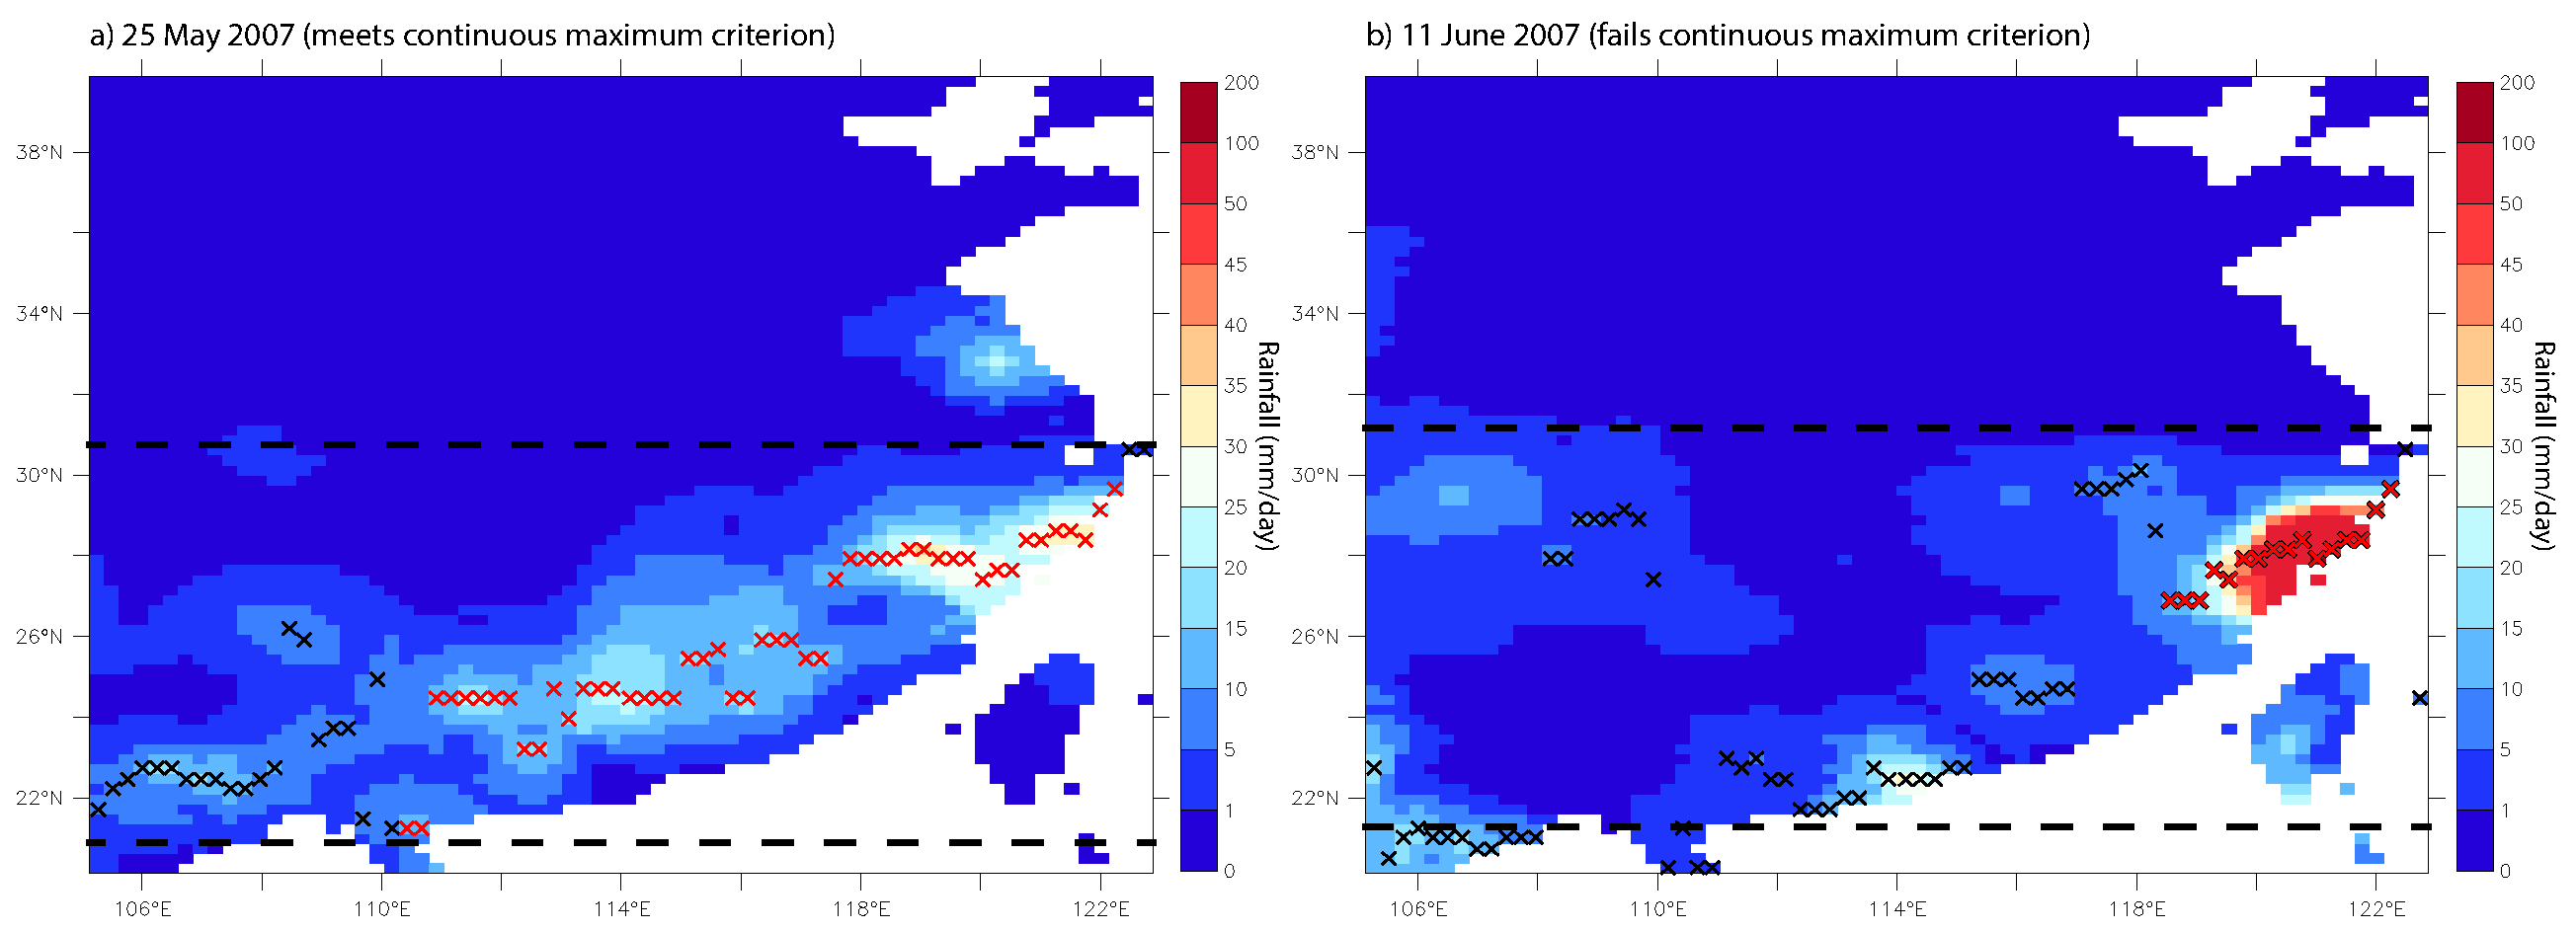
\includegraphics[width=36pc]{Figures/S1}
\caption{The first step of the Meiyu algorithm checks to see whether a five-degree continuous band of precipitation maxima above 10 mm day$^{-1}$ exists. If so, a fit of a frontal event is attempted. a) 25 May 2007 - the continuous maximum criterion is met and a fit is attempted. b) 11 June 2007 - although there is abundant rainfall in some locations, it appears not to be frontal and the continuous maximum criterion is failed. No fit is attempted.}
\end{figure}

%S2 - How the convergent fit algorithm works.
\begin{figure}
\setfigurenum{S2} %%Change number for each figure

\noindent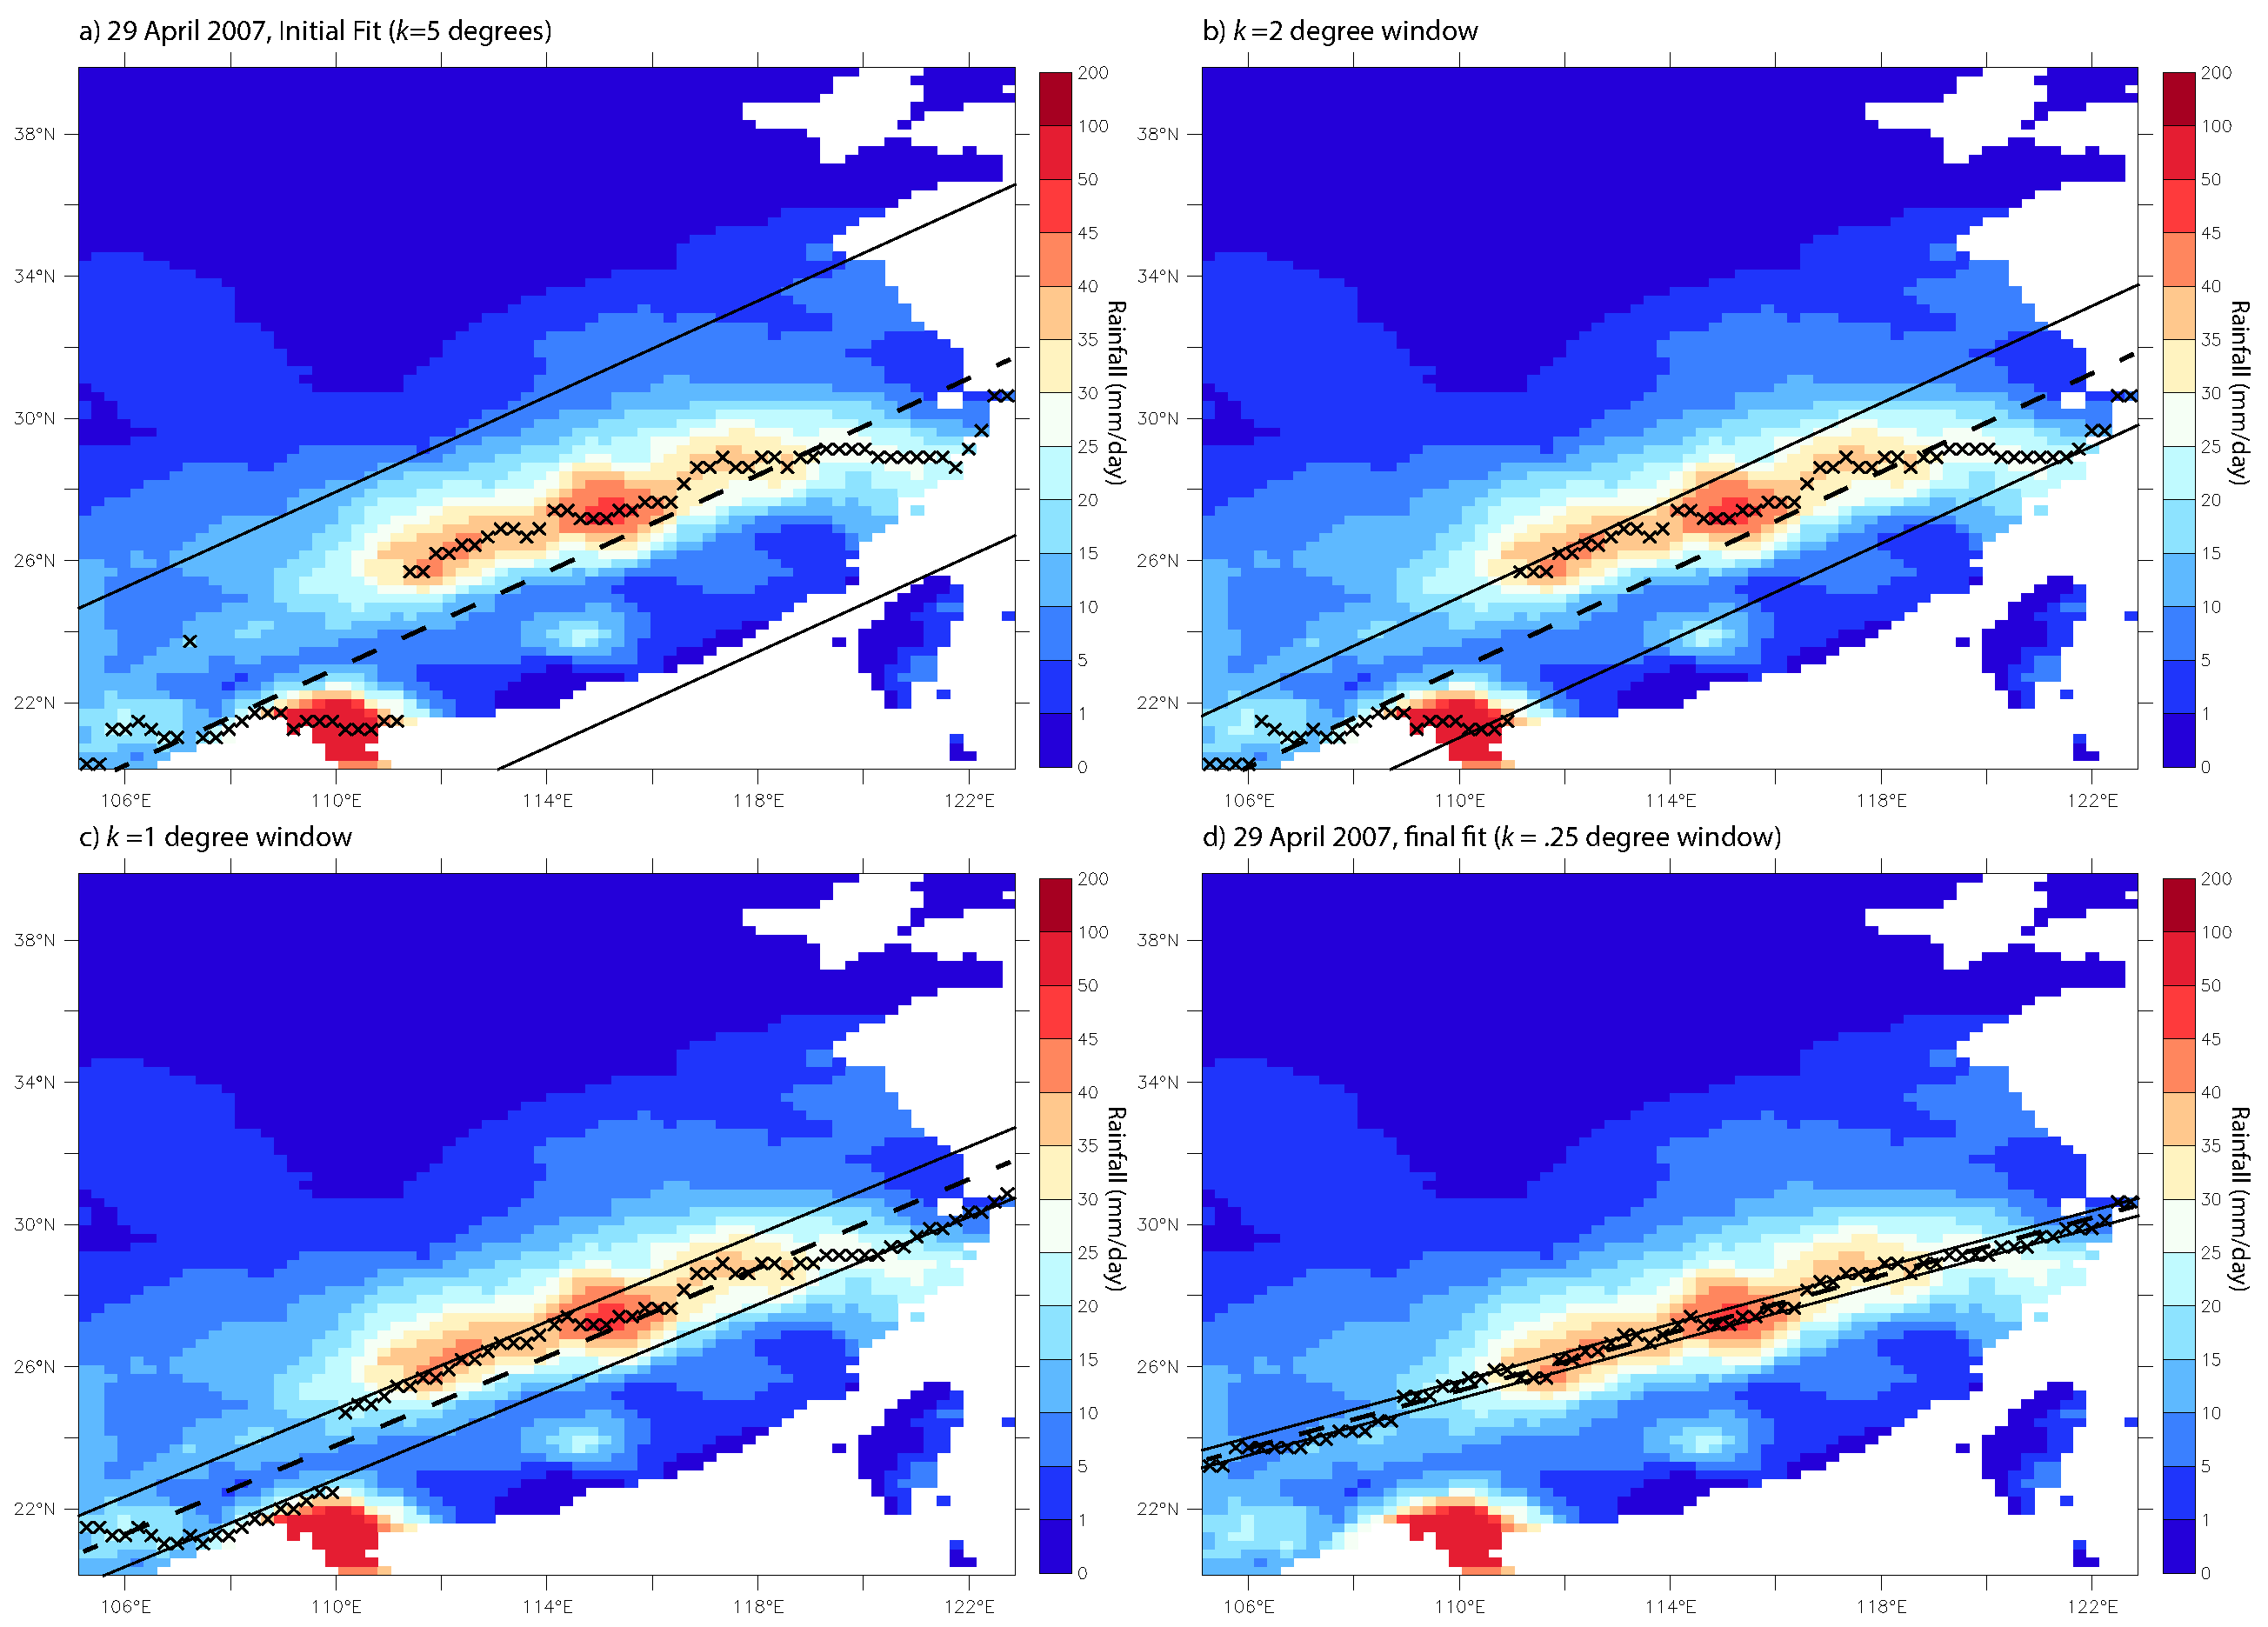
\includegraphics[width=36pc]{Figures/S2}
\caption{Display of the functionality of the recursive convergent algorithm. On 29 April 2007, a strong maximum in southernmost China skews our initial frontal fit (panel a), but the algorithm eventually converges on the most prominent coherent band via tighter windowing (panel d).}
\end{figure}

%S3 - Procedure for finding double front cases.
\begin{figure}
\setfigurenum{S3} %%Change number for each figure

\noindent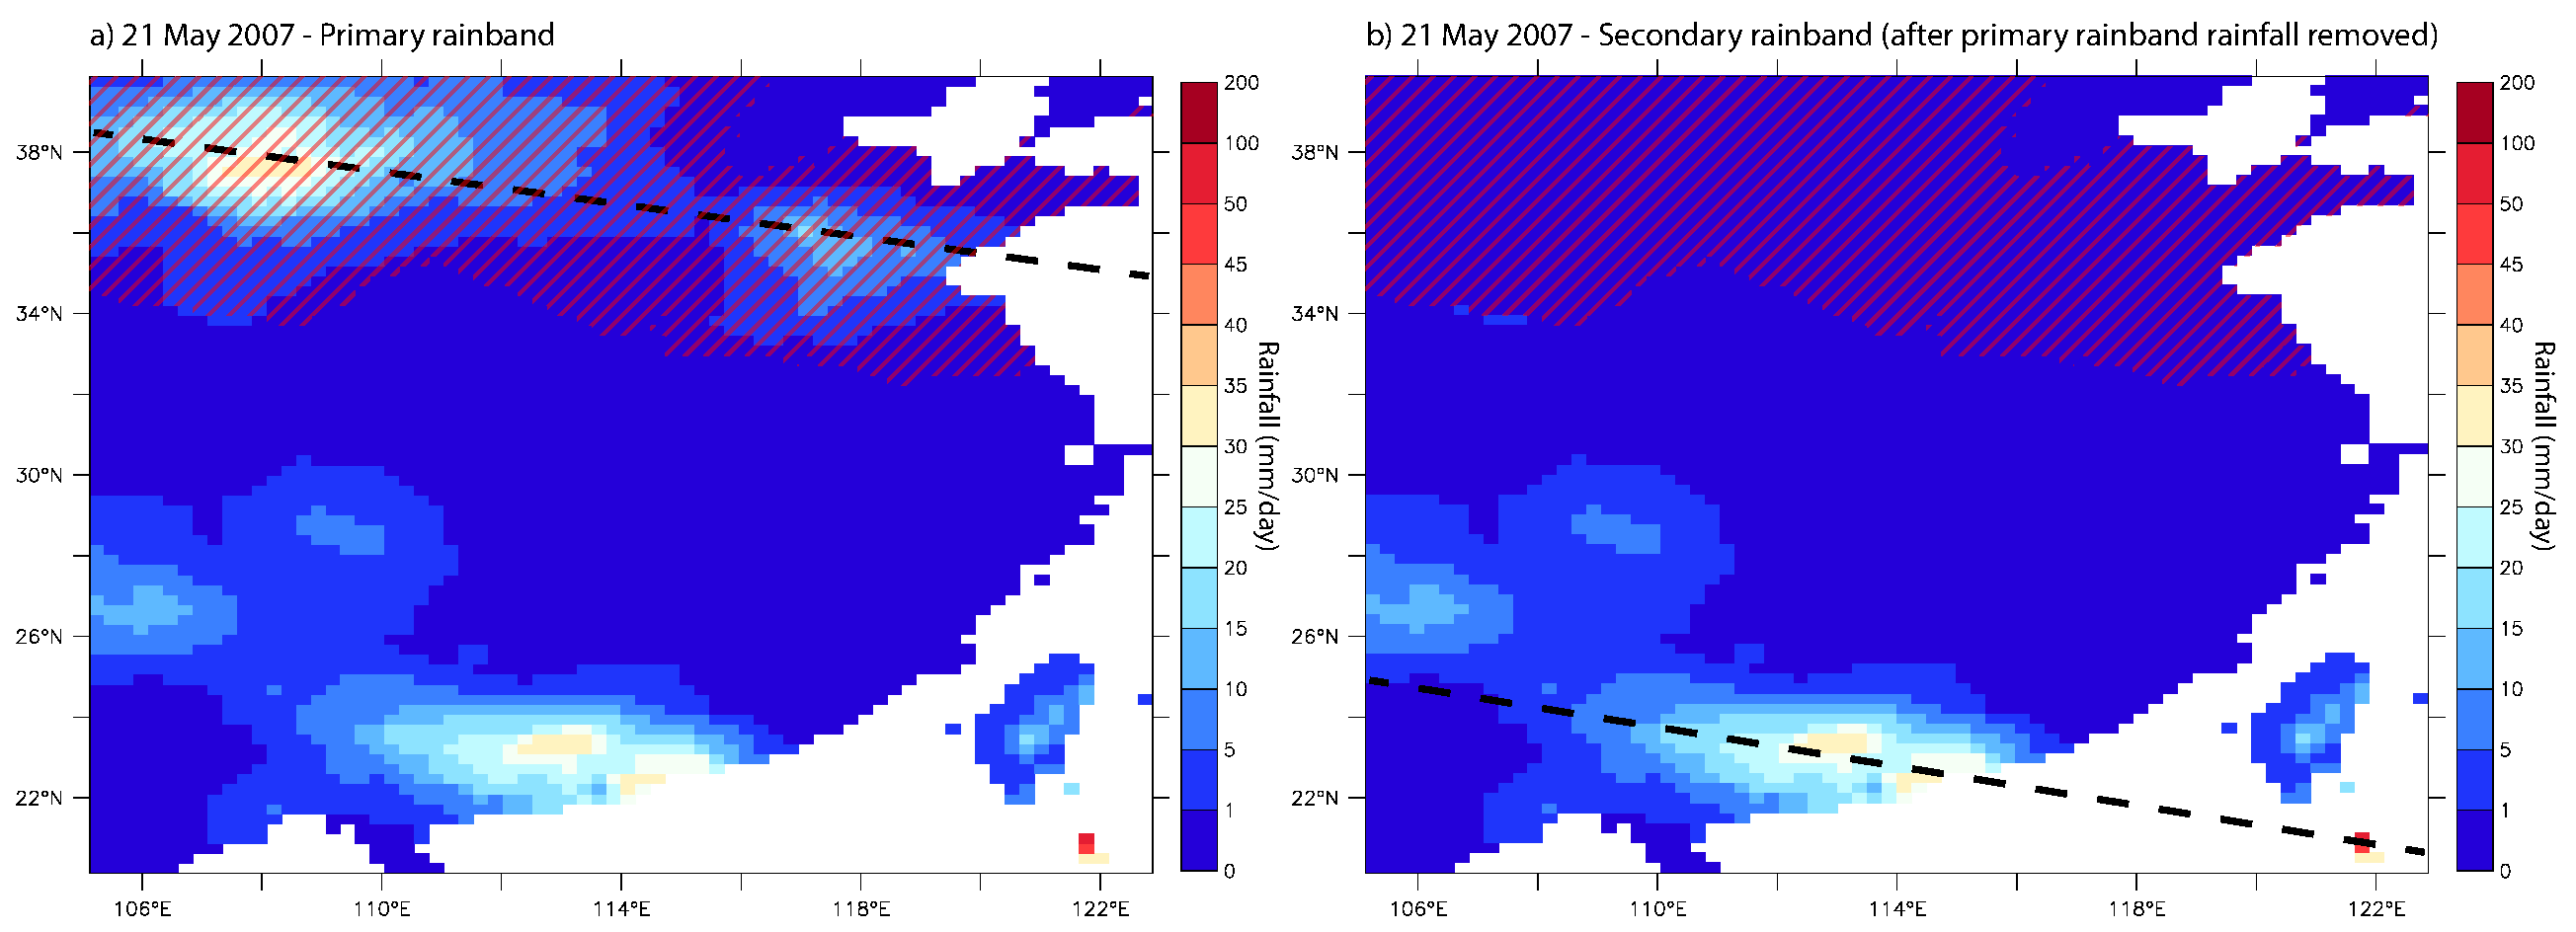
\includegraphics[width=36pc]{Figures/S3}
\caption{a) The algorithm converges on the strongest front, around 37N (defined as the ``primary front''). b) The rainfall associated with the primary front is removed, and we check for the presence of another front (a ``secondary front''), again using the continuous maximum criterion.}
\end{figure}

%S4 - Quality Control algorithm used to determine inclusion in statistics
\begin{figure}
\setfigurenum{S4} %%Change number for each figure

\noindent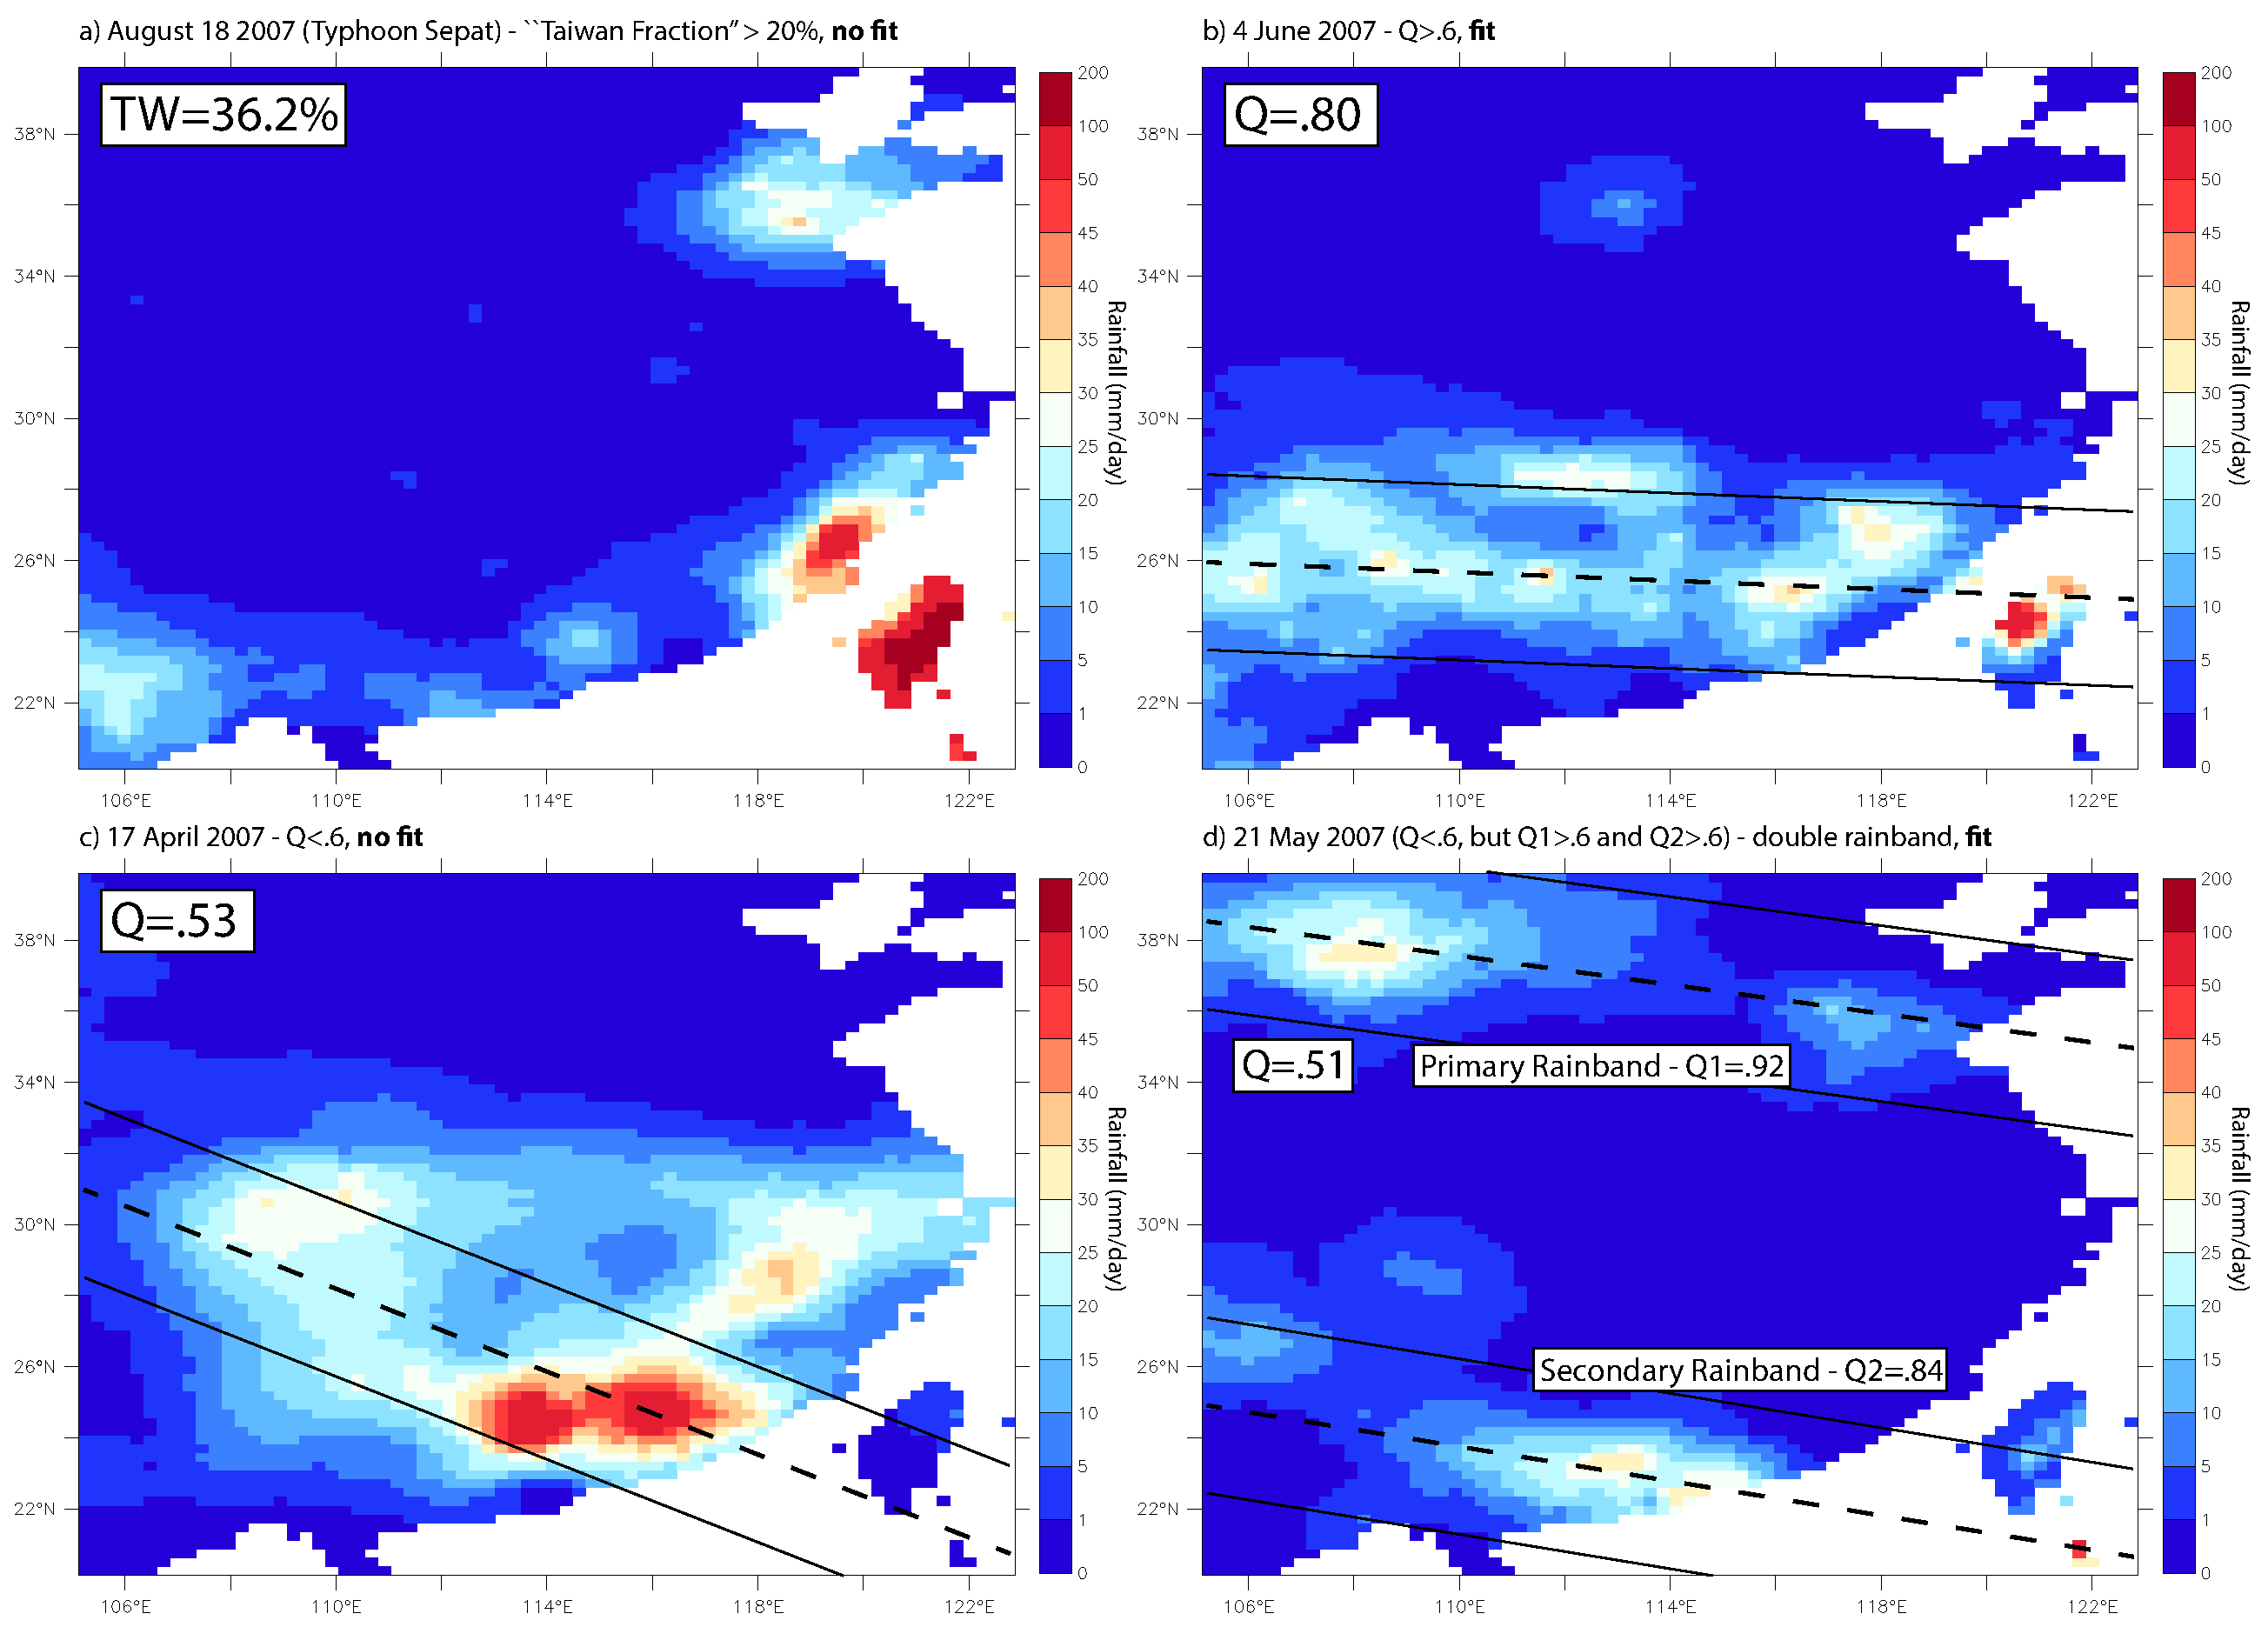
\includegraphics[width=36pc]{Figures/S4}
\caption{A Quality Control algorithm is used to weed out poor fits. a) 18 August 2007 - Days with a high Taiwan fraction (here, corresponding to the passage of Typhoon Sepat) are excluded from our statistics. b) June 4 2007 - A high-quality fit is achieved. c) 17 April 2007 - Although a fit is reached, it explains the distribution of daily rainfall poorly and is therefore excluded from frontal statistics. d) 21 May 2007 (same as Figure S3) - An initial fit appears to be of poor quality (Q1<.6). However, after finding a secondary front, we determine that conditional quality scores Q1 and Q2 are high, and the day is included in our statistics.}
\end{figure}

%S5 - Autocorrelation of jet during Pre-Meiyu and Post-Meiyu
\begin{figure}
\setfigurenum{S5} %%Change number for each figure

\noindent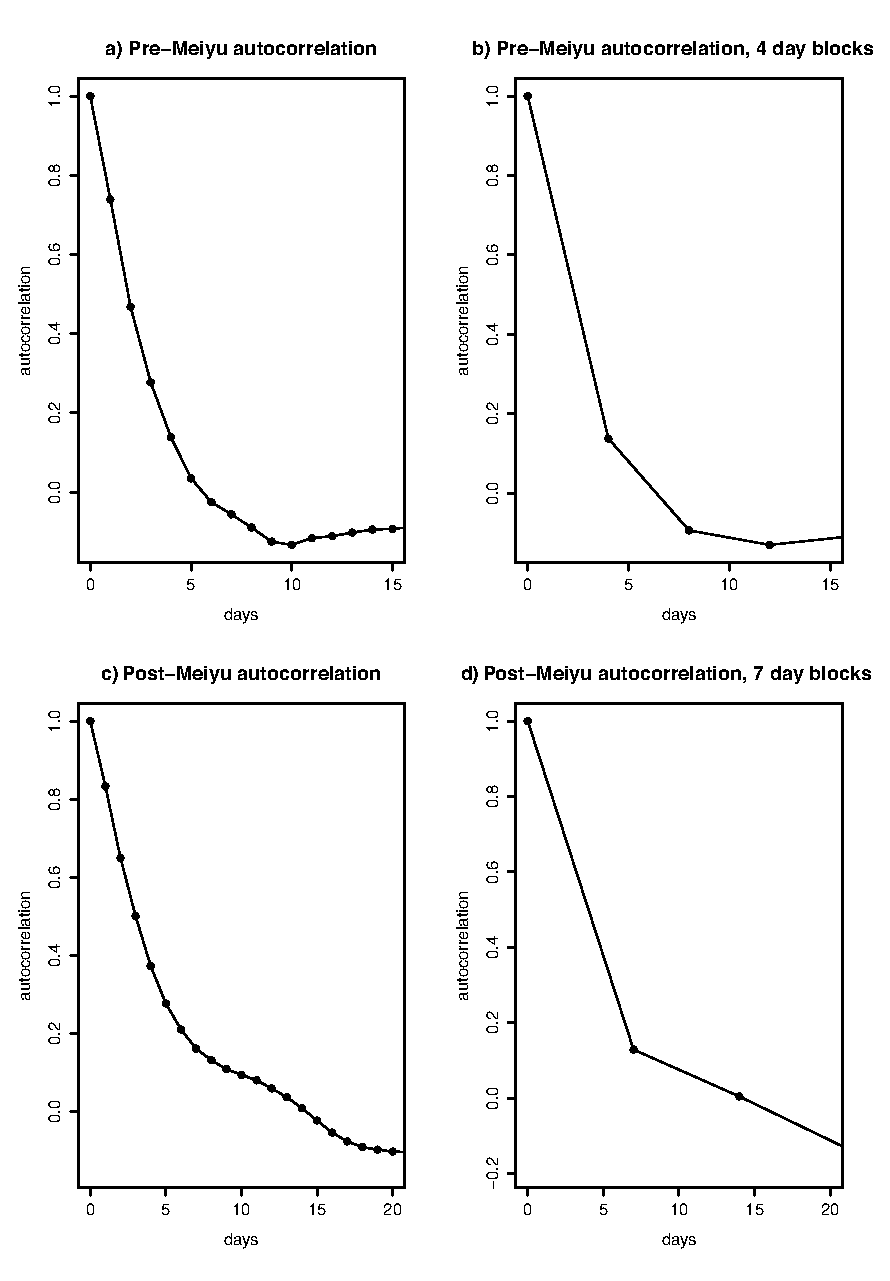
\includegraphics[width=36pc]{Figures/S5}
\caption{Autocorrelation of the jet during the Pre-Meiyu season (days 121-160) for a) daily and b) 4-day blocks; and during the Post-Meiyu season (days 201-273) for c) daily and d) 7-day blocks. The compiling of daily mean jet data into longer blocks removes temporal autocorrelation, which allows for the use of the Kolmogorov-Smirnov test. Panel c) shows that the autocorrelation of mean daily jet latitude is longer during the Post-Meiyu than during the Pre-Meiyu.}
\end{figure}

\end{article}

\end{document}



%% ------------------------------------------------------------------------ %%
%%  REFERENCE LIST AND TEXT CITATIONS
%
% Either type in your references using
% \begin{thebibliography}{}
% \bibitem{}
% Text
% \end{thebibliography}
%
% Or,
%
% If you use BiBTeX for your references, please use the agufull08.bst file (available at % ftp://ftp.agu.org/journals/latex/journals/Manuscript-Preparation/) to produce your .bbl
% file and copy the contents into your paper here.
%
% Follow these steps:
% 1. Run LaTeX on your LaTeX file.
%
% 2. Make sure the bibliography style appears as \bibliographystyle{agufull08}. Run BiBTeX on your LaTeX
% file.
%
% 3. Open the new .bbl file containing the reference list and
%   copy all the contents into your LaTeX file here.
%
% 4. Comment out the old \bibliographystyle and \bibliography commands.
%
% 5. Run LaTeX on your new file before submitting.
%
% AGU does not want a .bib or a .bbl file. Please copy in the contents of your .bbl file here.

%\begin{thebibliography}{}

%\providecommand{\natexlab}[1]{#1}
%\expandafter\ifx\csname urlstyle\endcsname\relax
%  \providecommand{\doi}[1]{doi:\discretionary{}{}{}#1}\else
%  \providecommand{\doi}{doi:\discretionary{}{}{}\begingroup
%  \urlstyle{rm}\Url}\fi
%
%\bibitem[{\textit{Atkinson and Sloan}(1991)}]{AtkinsonSloan}
%Atkinson, K., and I.~Sloan (1991), The numerical solution of first-kind
%  logarithmic-kernel integral equations on smooth open arcs, \textit{Math.
%  Comp.}, \textit{56}(193), 119--139.
%
%\bibitem[{\textit{Colton and Kress}(1983)}]{ColtonKress1}
%Colton, D., and R.~Kress (1983), \textit{Integral Equation Methods in
%  Scattering Theory}, John Wiley, New York.
%
%\bibitem[{\textit{Hsiao et~al.}(1991)\textit{Hsiao, Stephan, and
%  Wendland}}]{StephanHsiao}
%Hsiao, G.~C., E.~P. Stephan, and W.~L. Wendland (1991), On the {D}irichlet
%  problem in elasticity for a domain exterior to an arc, \textit{J. Comput.
%  Appl. Math.}, \textit{34}(1), 1--19.
%
%\bibitem[{\textit{Lu and Ando}(2012)}]{LuAndo}
%Lu, P., and M.~Ando (2012), Difference of scattering geometrical optics
%  components and line integrals of currents in modified edge representation,
%  \textit{Radio Sci.}, \textit{47},  RS3007, \doi{10.1029/2011RS004899}.

%\end{thebibliography}

%Reference citation examples:

%...as shown by \textit{Kilby} [2008].
%...as shown by {\textit  {Lewin}} [1976], {\textit  {Carson}} [1986], {\textit  {Bartholdy and Billi}} [2002], and {\textit  {Rinaldi}} [2003].
%...has been shown [\textit{Kilby et al.}, 2008].
%...has been shown [{\textit  {Lewin}}, 1976; {\textit  {Carson}}, 1986; {\textit  {Bartholdy and Billi}}, 2002; {\textit  {Rinaldi}}, 2003].
%...has been shown [e.g., {\textit  {Lewin}}, 1976; {\textit  {Carson}}, 1986; {\textit  {Bartholdy and Billi}}, 2002; {\textit  {Rinaldi}}, 2003].

%...as shown by \citet{jskilby}.
%...as shown by \citet{lewin76}, \citet{carson86}, \citet{bartoldy02}, and \citet{rinaldi03}.
%...has been shown \citep{jskilbye}.
%...has been shown \citep{lewin76,carson86,bartoldy02,rinaldi03}.
%...has been shown \citep [e.g.,][]{lewin76,carson86,bartoldy02,rinaldi03}.
%
% Please use ONLY \citet and \citep for reference citations.
% DO NOT use other cite commands (e.g., \cite, \citeyear, \nocite, \citealp, etc.).

%% ------------------------------------------------------------------------ %%
%
%  END ARTICLE
%
%% ------------------------------------------------------------------------ %%


